\newpage
\section{Diagramas de secuencia}
A continuación se describe la interacción de nuestras entidades de negocio y el ciclo de vida que tendrán en la aplicación. También se detalla la interacción,mensajes y la lógica implementada por cada uno de los diferentes escenarios.\par
\subsection{Registro}
El registro de un usuario nuevo consiste en capturar el correo, nombre y una contraseña. Esta captura sera tratada como un JSON el cual viajara atravéz de un método POST. Gateway se encargara de redirigir esta petición al servicio de registro. Este servicio viajara hacia RDS donde se enviara un INSERT para registrar los datos. 
\vspace{5mm}
\begin{figure}[h!]
	\centering
	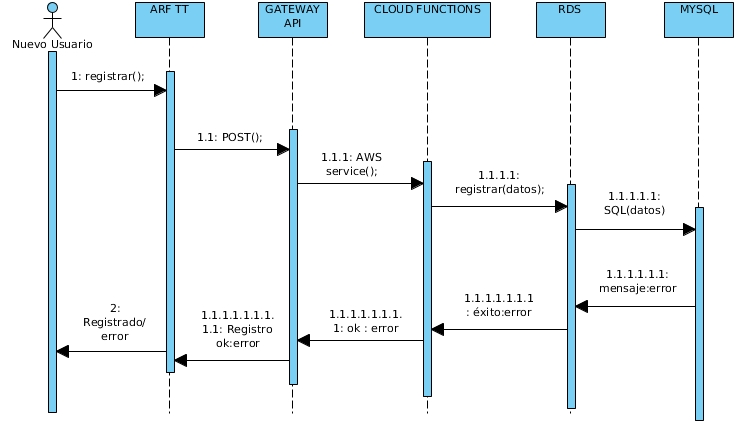
\includegraphics[width=14cm,height=8cm]{imagenes/analisis/DSregistrarUsuario.jpg}
	\caption{Diagrama de secuencia - Registrar usuario.}
	\label{fig:analogo}
\end{figure} 
\vspace{5mm}\par
Si el usuario y la contraseña se encuentra repetido, se enviara un mensaje de error, como se muestra en la figura 3.7
\newpage
\subsection{Login}
<<<<<<< HEAD
La validación de credenciales comienza con capturar el correo y contraseña  de un usuario registrado. Esta información sera tratada como un objeto JSON, el cual se mandara por una método POST. La API Gateway direccionara la petición a un Servicio AWS y  comparara la información en la instancia creada en RDS de un motor de base de datos MySQL. RDS se encargara de generar la conexión y consulta a la base de datos.
\vspace{5mm}
=======
La validación de credenciales comienza con capturar el correo y contraseña  de un usuario registrado. Esta información sera tratada como un objeto JSON, el cual se mandara por una método POST. La API Gateway direccionara la petición a un Servicio AWS y  comparará la información en la instancia creada en RDS de un motor de base de datos MySQL. RDS se encargara de generar la conexión y consulta a la base de datos. La petición regresara con un mensaje si hubo coincidencia, de lo contrario se enviara un error a la interfaz de usuario.
>>>>>>> 7cbf0b9ca67fe90765ccdb47c810557903007531
\begin{figure}[h!]
	\centering
	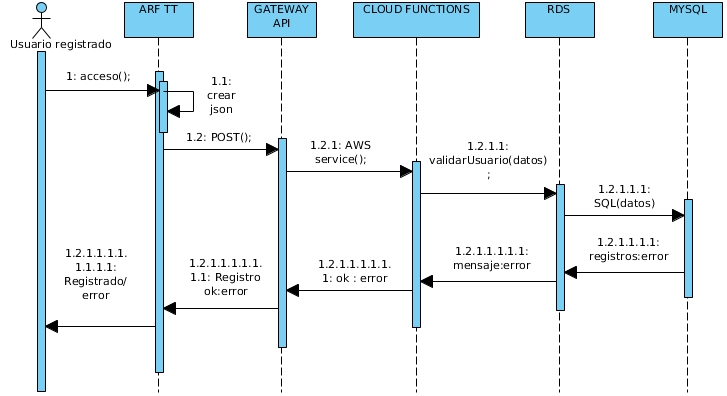
\includegraphics[width=14cm,height=8cm]{imagenes/analisis/DSacceso.jpg}
	\caption{Diagrama de secuencia - Registrar Acceso.}
	\label{fig:analogo}
\end{figure} 
\vspace{5mm} \par
La petición regresara con un mensaje si hubo coincidencia, de lo contrario se enviara un error a la interfaz de usuario.
\newpage
\subsection{Recuperar contraseña}\par
La recuperación de credenciales inicia con la función recuperar, en ella se captura el correo de un usuario y posteriormente lo procesa a un objeto JSON. Esta información se mandara en un método POST. La API Gateway envía la petición a un Servicio AWS y en la instancia creada en RDS procesa un script que comparara el correo con la  información de MySQL, buscando alguna coincidencia. Si existe una coincidencia exacta, MySQL enviará el registro en un mensaje con la contraseña.
\vspace{5mm}
\begin{figure}[h!]
	\centering
	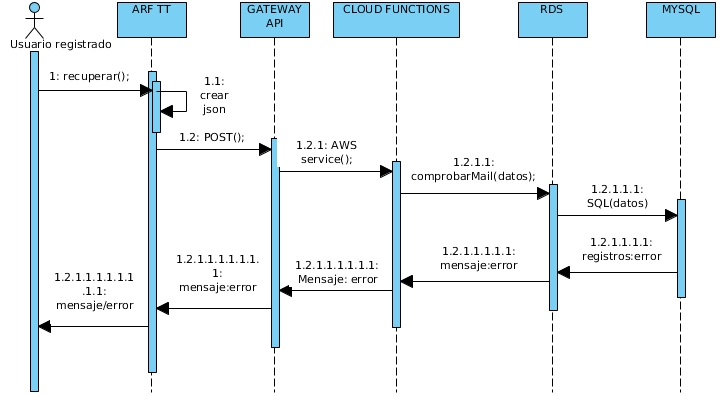
\includegraphics[width=14cm,height=8cm]{imagenes/analisis/DSrecuperarContra.jpg}
	\caption{Diagrama de secuencia - Recuperar contraseña.}
	\label{fig:analogo}
\end{figure}
\vspace{5mm} \par
Si no existe coincidencia se manda un mensaje de error. RDS se encargara de generar la conexión y consulta con el servicio de Amazon Web Services y nuestra instancia de MySQL en RDS.
\newpage
\subsection{Gestión de muebles}
La visualización y edición del color de un mueble inicia desde un menú con los muebles disponibles, cuando un actor selecciona un mueble este dispara una acción donde opcionalmente podrá editar el color. El actor después de seleccionar un color valido enviara la información a los servicios AWS donde se tienen almacenados los muebles, esta información será enviada de regreso para visualizar este objeto con la realidad aumentada de la aplicación.
\vspace{5mm}
\begin{figure}[h!]
	\centering
	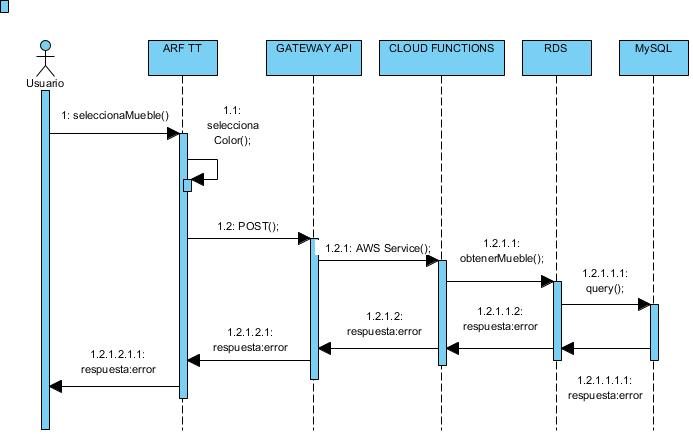
\includegraphics[width=14cm,height=8cm]{imagenes/analisis/DSgestionMuebles.jpg}
	\caption{Diagrama de secuencia -Gestión de muebles.}
	\label{fig:analogo}
\end{figure}
\vspace{5mm} \par
Si ocurre un error desde el servidor se envía un código de error donde se notificara al usuario que no se encuentra disponible.
\newpage
\subsection{Guardar escenario}
La creación y guardado de un escenario inicia cuando se comienza a capturar la realidad aumentada de un mueble, la acción que dispara este proceso será la de guardar escenario, la función tiene como parámetros el identificador del usuario, el nombre del escenario y una colección de imágenes en formato Base64. Esta función procesa las imágenes a binario para su posterior persistencia en S3 Bucket (Simple Storage Service).
\vspace{5mm}
\begin{figure}[h!]
	\centering
	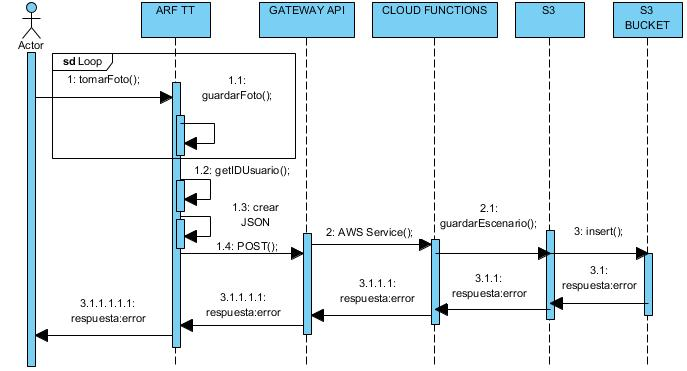
\includegraphics[width=14cm,height=8cm]{imagenes/analisis/DSguardarEscenario.jpg}
	\caption{Diagrama de secuencia - Guardar escenario.}
	\label{fig:analogo}
\end{figure}
\vspace{5mm}\par
El S3 envia un mensaje de éxito o error de la persistencia, el usuario observara la notificación de guardado satisfactorio. En dado caso que la petición sea incorrecta se enviara una notificación de guardado fallído.
\newpage
\subsection{Visualizar escenario}
La visualización de un escenario se dispara cuando el actor selecciona la opción visualizar escenario. La petición se envía por los servicios de AWS que consulta el bucket S3, este a su vez hace la consulta de la información con MySQL, si encuentra una coincidencia se obtiene los nombres y las URL de las imágenes guardadas. Esta información viaja de regreso para que sea visualizada en la pantalla de la aplicación.
\vspace{5mm}
\begin{figure}[h!]
	\centering
	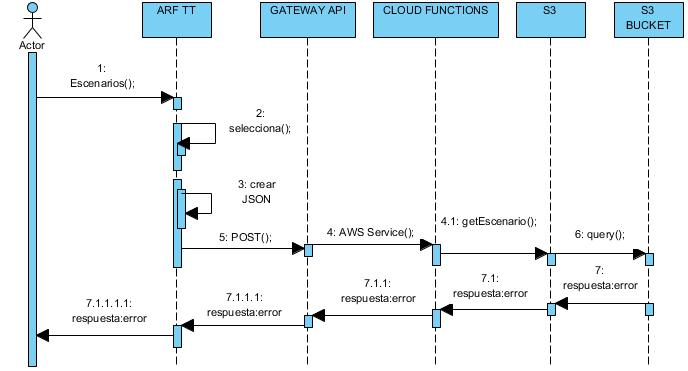
\includegraphics[width=14cm,height=8cm]{imagenes/analisis/DSvisualizarEscenario.jpg}
	\caption{Diagrama de secuencia - Visualizar escenario.}
	\label{fig:analogo}
\end{figure} 
\vspace{5mm} \par 
Si la petición no encuentra alguna coincidencia dentro de S3 se envía un código de error, informando que no existen escenarios para visualizar.



